\documentclass[../notes.tex]{subfiles}

\pagestyle{main}
\renewcommand{\chaptermark}[1]{\markboth{\chaptername\ \thechapter\ (#1)}{}}
\renewcommand{\thechapter}{\Roman{chapter}}
\setcounter{chapter}{7}

\begin{document}




\chapter{Electronic Spectra of Coordination Compounds}
\section{Module 40: Electronic Transitions}
\begin{itemize}
    \item \marginnote{3/1:}Suggested reading: Chapter 11.1.
    \item Transition metal complexes are known to show rich photophysics and optical properties.
    \begin{itemize}
        \item For example, \ce{[Ni(NH3)6]^2+} has peaks in the infrared, visible, and UV spectra.
    \end{itemize}
    \item How electronic transitions occur:
    \begin{itemize}
        \item Take a solid or aqueous sample and illuminate it with photons of a particular power/intensity $P_0$ through $l\si{\centi\meter}$ of it.
        \item Some will be absorbed and some will pass through. Measure the power $P$ that comes out on the other side.
    \end{itemize}
    \item Transmittance $T=P/P_0$.
    \item Absorbance $A=-\log T=\log\frac{P_0}{P}$.
    \item The Beer-Lambert Law: $A=\varepsilon Cl$, where $C$ is the concentration of the sample in solution, $l$ is the path length (the length through solution), and $\varepsilon$ is the molar absorption coefficient.
    \item Plotting the wavelength of the impinging photons vs. $\varepsilon$ gives us a graph with peaks, where each peak corresponds to an electron transition.
    \item Spectral features:
    \begin{itemize}
        \item Number of transitions.
        \item Energy of the transitions.
        \item Intensity of the transitions.
        \item Shape of the transition.
    \end{itemize}
    \item \textbf{Transition probability}: The probability of a particular transition taking place.
    \item The transition probability depends on:
    \begin{itemize}
        \item Energy of the transition vs. incident light.
        \item Orientation of the molecule/material.
        \item Symmetry of the initial and final states.
        \item Angular momentum (spin).
    \end{itemize}
    \item The absorption spectra of various hexaaqua complexes of the first-row transition metals give us a zoo of spectra.
    \item We usually have $\varepsilon<10$, which means faint colors.
    \item Types of molecular transitions:
    \begin{itemize}
        \item Metal Centered (MC): Transitions between the $d$-orbitals on the metal center.
        \item Ligand to Metal Charge Transfer (LMCT): For example, \ce{MnO4-} has $\varepsilon\approx\num{10000}$.
        \item Metal to Ligand Charge Transfer (MLCT) and Metal to Metal Charge Transfer (MMCT), too.
    \end{itemize}
    \item The transition probability of one molecule from one state $\Psi_1$ to another state $\Psi_2$ is given by $|\vec{M}_{21}|$, the transition dipole moment or transition moment from $\Psi_1$ to $\Psi_2$.
    \begin{itemize}
        \item The transition matrix element $\vec{M}_{21}=\int\Psi_2\vec{\mu}\Psi_1\dd{\tau}$, where $\vec{\mu}$ is the electric dipole moment operator $\vec{\mu}=\sum_nQ_n\vec{x}_n$, where $Q_n$ is charge and $\vec{x}_n$ is the position vector operator.
        \item Derived with time-dependent perturbation theory.
        \item For an electronic transition to be allowed, the transition moment integral must be nonzero.
        \item Note that $\varepsilon\approx\vec{M}_{21}$.
    \end{itemize}
    \item How the HOMO moves about the molecule depends on the type of incoming light.
    \begin{itemize}
        \item If $\vec{M}_{21}=0$, then the transition probability is 0 and the transition from $\Psi_1$ to $\Psi_2$ is forbidden or electric-dipole forbidden ($\varepsilon=0$).
        \item If $\vec{M}_{21}\neq 0$, then the transition probability is not 0 and the transition from $\Psi_1$ to $\Psi_2$ is not forbidden ($\varepsilon\geq 0$).
        \begin{itemize}
            \item If $\vec{M}_{21}\neq 0$, we do not definitively know that there will be an electron transition or know how intense it will be; we just know that it is not electric-dipole forbidden.
        \end{itemize}
    \end{itemize}
    \item Calculating $\vec{M}_{21}$:
    \begin{itemize}
        \item Use the same procedure with $\Gamma_2\otimes\Gamma_\mu\otimes\Gamma_1$ as in Module 12.
        \item If the direct product does not contain the totally symmetric representation, then the transition is forbidden by symmetry arguments.
        \item If the direct product does contain the totally symmetric representation, then the transition is allowed by symmetry arguments.
    \end{itemize}
    \begin{table}[h!]
        \centering
        \small
        \renewcommand{\arraystretch}{1.4}
        \begin{tabular}{|c|lll|}
            \hline
            \normalsize$C_{3v}$ & $\bm{A_1}$ & $\bm{A_2}$ & \multicolumn{1}{c|}{$\bm{E}$}\\
            \hline
            $\bm{A_1}$ & $A_1$ & $A_2$ & $E$\\
            $\bm{A_2}$ &       & $A_1$ & $E$\\
            $\bm{E}$   &       &       & $A_1+[A_2]+E$\\
            \hline
        \end{tabular}
        \caption{Direct product table for the $C_{3v}$ point group.}
        \label{tab:directProductTable-C3v}
    \end{table}
    \item Be aware of direct product tables, such as the above example, which we may readily obtain from Table \ref{tab:characterTable-C3v}.
    \item Example: In a $D_{2h}$ complex, can we excite a $d_{z^2}$ electron to the $p_z$ orbital?
    \begin{itemize}
        \item From the $D_{2h}$ character table, we have that $\Gamma_1=A_g$ and $\Gamma_2=B_{1u}$. We also have that $\Gamma_\mu$ for an $x$-, $y$-, and $z$-basis is $B_{3u}$, $B_{2u}$, and $B_{1u}$, respectively.
        \item Taking direct products under each basis gives us
        \begin{align*}
            B_{1u}\otimes B_{3u}\otimes A_g &= B_{2g}\tag{$x$-basis}\\
            B_{1u}\otimes B_{2u}\otimes A_g &= B_{3g}\tag{$y$-basis}\\
            B_{1u}\otimes B_{1u}\otimes A_g &= A_g\tag{$z$-basis}
        \end{align*}
        \item Thus, the $x$- and $y$-components are forbidden while the $z$ one is not.
        \item What this means is that $z$-plane polarized light will be able to cause the desired electron transition, but $x$- and $y$-plane polarized light will not.
    \end{itemize}
    \item We can use the same procedure to prove that we can never promote an electron from $d_{xy}$ to $p_z$.
    \item We can use the same procedure for octahedral complexes, except the calculations of the direct products are just a bit more difficult.
    \begin{itemize}
        \item For a $d^1$ complex, we calculate $E_g\otimes T_{1u}\otimes T_{2g}$.
        \item For a $d^6$ complex, we calculate $(T_{2g}\otimes E_g)\otimes T_{1u}\otimes A_{1g}=(T_{1g}+T_{2g})\otimes T_{1u}\otimes A_{1g}$.
        \begin{itemize}
            \item A low spin $d^6$ complex has $A_{1g}$ symmetry by taking the direct product of $T_{2g}$ times itself six times.
            \item The excited state has $T_{2g}$ times itself five times, and then times $E_g$.
            \item Basically, we take the direct product of the orbital that each electron occupies.
        \end{itemize}
    \end{itemize}
\end{itemize}



\section{Module 41: Many Electron States}
\begin{itemize}
    \item Suggested reading: Chapter 11.2.
    \item For octahedral $d^3$, we have multiple excited states (six, to be exact).
    \begin{itemize}
        \item Fortunately, there is an easier way to describe transitions between states (we will talk about this next time).
    \end{itemize}
    \item A single electron is completely described by the principal quantum number $n$, its angular momentum $\ell$, its magnetic quantum number $m_\ell$, and its spin $m_s$.
    \item Multielectron states are described by \textbf{Russell-Saunders coupling}, \emph{also known as} \textbf{LS coupling}, \textbf{L-S coupling}.
    \item For example, consider the $d^2$ configured \ce{V^3+} ion.
    \begin{itemize}
        \item There are 45 different possible microstates. Some will have the same energy, some will not.
        \item There are five states (denoted by \textbf{term symbols}) with distinct energy in total.
    \end{itemize}
    \item To find the term symbol, we need:
    \begin{itemize}
        \item $L=\text{total orbital angular momentum}=\sum m_\ell$.
        \item $S=\text{total spin angular momentum}=\sum m_s$.
    \end{itemize}
    \item Term symbols then are of the form
    \begin{equation*}
        {}^{2S+1}L_J
    \end{equation*}
    where $2S+1$ is the spin multiplicity, $L$ is the subshell letter corresponding to the angular momentum quantum number ($0\mapsto s$, $1\mapsto p$, $2\mapsto d$, $3\mapsto f$, \dots), and $J$ is the total angular momentum ($J=L+S,L+S-1,L+S-2,\dots,|L-S|$, the spin-orbit coupling).
    \item Some examples:
    \begin{itemize}
        \item \tikz[xscale=1.5,every node/.append style={black},baseline={(0,0)}]{\footnotesize\draw [gry,ultra thick] (0,0) -- node{\Large$\upharpoonleft$} node[below=2mm]{$+1/2$} ++(0.5,0) ++(0.1,0) -- ++(0.5,0) ++(0.1,0) -- ++(0.5,0) ++(0.1,0) -- ++(0.5,0) ++(0.1,0) -- ++(0.5,0)}: $S=\frac{1}{2}$, so our term symbol will be of the form ${}^2L_J$\footnote{Pronounced "doublet state."}.
        \item \tikz[xscale=1.5,every node/.append style={black},baseline={(0,0)}]{\footnotesize\draw [gry,ultra thick] (0,0) -- node{\Large$\upharpoonleft$} node[below=2mm]{$+1/2$} ++(0.5,0) ++(0.1,0) -- node{\Large$\upharpoonleft$} node[below=2mm]{$+1/2$} ++(0.5,0) ++(0.1,0) -- node{\Large$\downharpoonright$} node[below=2mm]{$-1/2$} ++(0.5,0) ++(0.1,0) -- node{\Large$\upharpoonleft$} node[below=2mm]{$+1/2$} ++(0.5,0) ++(0.1,0) -- ++(0.5,0)}: $S=1$, so our term symbol will be of the form ${}^3L_J$.
        \item \tikz[xscale=1.5,every node/.append style={black},baseline={(0,0)}]{\footnotesize\draw [gry,ultra thick] (0,0) -- node{\Large$\upharpoonleft$} node[below=2mm]{$+2$} ++(0.5,0) ++(0.1,0) -- node{\Large$\upharpoonleft$} node[below=2mm]{$+1$} ++(0.5,0) ++(0.1,0) -- node[below=2mm]{$0$} ++(0.5,0) ++(0.1,0) -- node[below=2mm]{$-1$} ++(0.5,0) ++(0.1,0) -- node[below=2mm]{$-2$} ++(0.5,0)}: $S=1$ and $L=3$, so our term symbol will be of the form ${}^3F_J$\footnote{Pronounced "triplet eff state."}.
        \item \tikz[xscale=1.5,every node/.append style={black},baseline={(0,0)}]{\footnotesize\draw [gry,ultra thick] (0,0) -- node{\Large$\upharpoonleft$} node[below=2mm]{$+2$} ++(0.5,0) ++(0.1,0) -- node[below=2mm]{$+1$} ++(0.5,0) ++(0.1,0) -- node[below=2mm]{$0$} ++(0.5,0) ++(0.1,0) -- node[below=2mm]{$-1$} ++(0.5,0) ++(0.1,0) -- node{\Large$\upharpoonleft$} node[below=2mm]{$-2$} ++(0.5,0)}: $S=1$ and $L=0$, so our term symbol will be of the form ${}^3S_J$\footnote{Pronounced "triplet ess state."}.
    \end{itemize}
    \item Spin-orbit coupling is weak for a carbon atom (we can essentially just disregard it).
    \begin{itemize}
        \item For lanthanides, it becomes very significant.
    \end{itemize}
    \item \marginnote{3/3:}In term symbols, $J$ is typically a small correction to the energy for light elements.
    \begin{itemize}
        \item It becomes significant with the lanthanides and actinides.
    \end{itemize}
    \item We group electrons into terms because each state has a characteristic energy in the absence of external electric and magnetic fields.
    \begin{itemize}
        \item If we do apply an external magnetic fields, states will split into $2S+1$ substates.
        \item Each term includes multiple microstates, which are atomic states produced by interactions of the atom with a magnetic field.
    \end{itemize}
    \item Consider the examples from above. The third and fourth examples are very similar but give rise to two different terms. This is because if we have ions with these states, we will observe differing energy levels spectroscopically.
    \item What if we have one electron in the orbital with $m_\ell=-2$? Then how do we create the term symbol?
    \begin{itemize}
        \item It is part of one of the microstates of the ${}^1D$ term.
        \item We fill electrons starting with the lowest energy states, and the lowest energy state has the greatest spin multiplicity (e.g., $+2$; this is one of Hund's rules).
    \end{itemize}
    \item Correspondences between $d$ electron configurations and term symbols:
    \begin{align*}
        d^1 &= {}^2D&
            d^6 &= {}^5D\\
        d^2 &= {}^3F&
            d^7 &= {}^4F\\
        d^3 &= {}^4F&
            d^8 &= {}^3F\\
        d^4 &= {}^5D&
            d^9 &= {}^2D\\
        d^5 &= {}^6S&
            d^{10} &= {}^1S\\
    \end{align*}
    \begin{itemize}
        \item Note that a fully occupied or unoccupied subshell is always ${}^1S$.
        \item Now if we take a direct product of a singlet $S$ state with any other state, we will have just that state left over. This implies that we can ignore all fully occupied shells, and the term will be determined entirely by partially filled ones.
    \end{itemize}
    \item If we want to build the full picture and see all possible states, we need a \textbf{microstate table}.
    \item Microstate table:
    \begin{itemize}
        \item A microstate table contains all possible combinations of $m_\ell$ and $m_s$.
        \item Each microstate represents a possible electron configuration.
        \item It includes both ground and excited states.
        \item It must obey the Pauli exclusion principle.
    \end{itemize}
    \item Example ($p^2$ electron configuration):
    \begin{itemize}
        \item Microstate notation:
        \begin{itemize}
            \item For each of the $n$ electrons in the configuration, list a special symbol in an $n$-tuple.
            \item The special symbol will be a number ($m_\ell$) with either a $+$ or $-$ sign as an exponent (for positive and negative spin, respectively).
        \end{itemize}
        \item There are three ground state configurations.
        \begin{itemize}
            \item \tikz[xscale=1.5,every node/.append style={black},baseline={(0,0)}]{\footnotesize\draw [gry,ultra thick] (0,0) -- node{\Large$\upharpoonleft$} node[below=2mm]{$+1$} ++(0.5,0) ++(0.1,0) -- node{\Large$\upharpoonleft$} node[below=2mm]{$0$} ++(0.5,0) ++(0.1,0) -- node[below=2mm]{$-1$} ++(0.5,0)}: The microstate is $(1^+,0^+)$.
            \item \tikz[xscale=1.5,every node/.append style={black},baseline={(0,0)}]{\footnotesize\draw [gry,ultra thick] (0,0) -- node[below=2mm]{$+1$} ++(0.5,0) ++(0.1,0) -- node{\Large$\upharpoonleft$} node[below=2mm]{$0$} ++(0.5,0) ++(0.1,0) -- node{\Large$\upharpoonleft$} node[below=2mm]{$-1$} ++(0.5,0)}: The microstate is $(0^+,-1^+)$.
            \item \tikz[xscale=1.5,every node/.append style={black},baseline={(0,0)}]{\footnotesize\draw [gry,ultra thick] (0,0) -- node{\Large$\upharpoonleft$} node[below=2mm]{$+1$} ++(0.5,0) ++(0.1,0) -- node[below=2mm]{$0$} ++(0.5,0) ++(0.1,0) -- node{\Large$\upharpoonleft$} node[below=2mm]{$-1$} ++(0.5,0)}: The microstate is $(1^+,-1^+)$.
        \end{itemize}
        \item We will not show all excited state configurations, but we will show a few.
        \begin{itemize}
            \item \tikz[xscale=1.5,every node/.append style={black},baseline={(0,0)}]{\footnotesize\draw [gry,ultra thick] (0,0) -- node{\Large$\upharpoonleft$\hspace{-1mm}$\downharpoonright$} node[below=2mm]{$+1$} ++(0.5,0) ++(0.1,0) -- node[below=2mm]{$0$} ++(0.5,0) ++(0.1,0) -- node[below=2mm]{$-1$} ++(0.5,0)}: The microstate is $(1^+,1^-)$.
            \item \tikz[xscale=1.5,every node/.append style={black},baseline={(0,0)}]{\footnotesize\draw [gry,ultra thick] (0,0) -- node[below=2mm]{$+1$} ++(0.5,0) ++(0.1,0) -- node{\Large$\upharpoonleft$\hspace{-1mm}$\downharpoonright$} node[below=2mm]{$0$} ++(0.5,0) ++(0.1,0) -- node[below=2mm]{$-1$} ++(0.5,0)}: The microstate is $(0^+,0^-)$.
            \item \tikz[xscale=1.5,every node/.append style={black},baseline={(0,0)}]{\footnotesize\draw [gry,ultra thick] (0,0) -- node[below=2mm]{$+1$} ++(0.5,0) ++(0.1,0) -- node[below=2mm]{$0$} ++(0.5,0) ++(0.1,0) -- node{\Large$\upharpoonleft$\hspace{-1mm}$\downharpoonright$} node[below=2mm]{$-1$} ++(0.5,0)}: The microstate is $(-1^+,-1^-)$.
        \end{itemize}
        \item We can now generate the microstate table.
        \begin{table}[h!]
            \centering
            \small
            \renewcommand{\arraystretch}{1.4}
            \begin{tabular}{c|c|c|c|c|}
                \multicolumn{2}{c}{} & \multicolumn{3}{c}{$M_S$}\\
                \cline{3-5}
                \multicolumn{2}{c|}{} & $-1$ & $0$ & $+1$\\
                \cline{2-5}
                 & $+2$ & & $1^+1^-$ & \\
                \cline{2-5}
                 & $+1$ & $1^-0^-$ & \vertcell{$1^+0^-$\\[-3pt]$1^-0^+$} & $1^+0^+$\\
                \cline{2-5}
                $M_L$ & $0$ & $-1^-1^-$ & \vertcell{$-1^+1^-$\\[-3pt]$0^+0^-$\\[-3pt]$-1^-1^+$} & $-1^+1^+$\\
                \cline{2-5}
                 & $-1$ & $-1^-0^-$ & \vertcell{$-1^+0^-$\\[-3pt]$-1^-0^+$} & $-1^+0^+$\\
                \cline{2-5}
                 & $-2$ & & $-1^+-1^-$ & \\
                \cline{2-5}
            \end{tabular}
            \caption{Microstate table for a $p^2$ electron configuration.}
            \label{tab:microstateTable-p2}
        \end{table}
        \begin{itemize}
            \item Each column represents a state with a given spin angular momentum.
            \item Each row represents the sum of the angular momentum of two electrons.
        \end{itemize}
        \item To analyze the microstate label, rename each microstate with $X$.
        \begin{itemize}
            \item Each term consists of multiple microstates of equivalent energies (similar to how we can have multiple degenerate orbitals of a given energy).
            \item We can lift degeneracy by applying an external electric (\textbf{Stark effect}) or magnetic field (\textbf{Ziemann effect}).
        \end{itemize}
        \item Now each term consists of $(2L+1)(2S+1)$ states (this is the \textbf{double multiplicity formula}).
        \item Group energetically equivalent states:
        \begin{itemize}
            \item First, focus on the term containing the states with the largest possible $L$ (i.e., those with $+2$). We know that it contains $(2(2)+1)(2(0)+1)=5$ microstates. Choose 5 microstates from the $M_S=0$ column, one per $M_L$.
            \item Next, focus on the term containing states with the next largest possible $L$ (i.e., those with $+1$ and $M_S=+1$). We know that it contains $(2(1)+1)(2(1)+1)=9$ microstates. Choose 9 microstates, one from each box in the square bounded by $(-1,-1)$ and $(+1,+1)$.
            \item The remaining microstate in $M_S=M_L=0$ forms its own term.
        \end{itemize}
        \item Thus, our microstate table can be decomposed into three terms (${}^1D$, ${}^3P$, and ${}^1S$).
    \end{itemize}
    \item Identifying relative energies with Hund's rules:
    \begin{itemize}
        \item For a given electron configuration, the term with the greatest spin multiplicity lies lowest in energy (Hund's rule).
        \item For a term with a given multiplicity, the greater the value of $L$, the lower the energy.
        \item Note that the rules for predicting the ground state always work, but they may fail in predicting the order of energies for excited states.
    \end{itemize}
    \item Thus, going back to our example, we have that energetically, ${}^3P<{}^1D<{}^1S$.
    \item Example ($d^2$ electron configuration):
    \begin{itemize}
        \item In this example, Hund's rules do not provide accurate energy predictions (they would predict ${}^3F<{}^3P<{}^1G<{}^1D<{}^1S$, but in reality, ${}^3F<{}^1D<{}^3P<{}^1G<{}^1S$).
    \end{itemize}
    \item \textbf{Electron-hole formalism}: The Russel-Saunders terms for $d^n$ and $d^{10-n}$ configurations are identical for $n=0,\dots,5$.
    \begin{itemize}
        \item We can rationalize this by thinking of $n$ electrons and $10-n$ holes (or positrons) as related to $10-n$ electrons and $n$ holes.
    \end{itemize}
\end{itemize}



\section{Module 42: Many Electron States and Transitions in Coordination Compounds}
\begin{itemize}
    \item Suggested reading: Chapter 11.3.
    \item Ligand field dependence ($d^1$ system):
    \begin{itemize}
        \item Degenerate symmetric field:
        \begin{itemize}
            \item Absence of ligand field.
            \item Free-ion term.
            \item All $d$-orbitals are energetically equal.
            \item If all $d$ orbitals are degenerate, then we can put a single electron in any orbital and we will have a microstate of ${}^2D$.
        \end{itemize}
        \item Infinite $O_h$ field:
        \begin{itemize}
            \item Strong ligand field.
            \item Coordination complexes.
            \item $d$-orbitals are not degenerate ($d_{z^2,x^2-y^2}$ have higher energy; $d_{xy,xz,yz}$ have lower energy).
            \item In this case, it matters in which $d$ orbital we put the electron.
        \end{itemize}
        \item Real molecules:
        \begin{itemize}
            \item We use a correlation diagram or Orgel diagram.
            \item If ligand field strength is zero, we have the degenerate symmetric field. If it is at maximum strength, we have two distinct states ($t_{2g}$ and $e_g$). Anywhere in between, the states are in between in energy, too (as we apply the ligand field, we split the state).
        \end{itemize}
    \end{itemize}
    \item Ligand field dependence ($d^2$ system):
    \begin{figure}[h!]
        \centering
        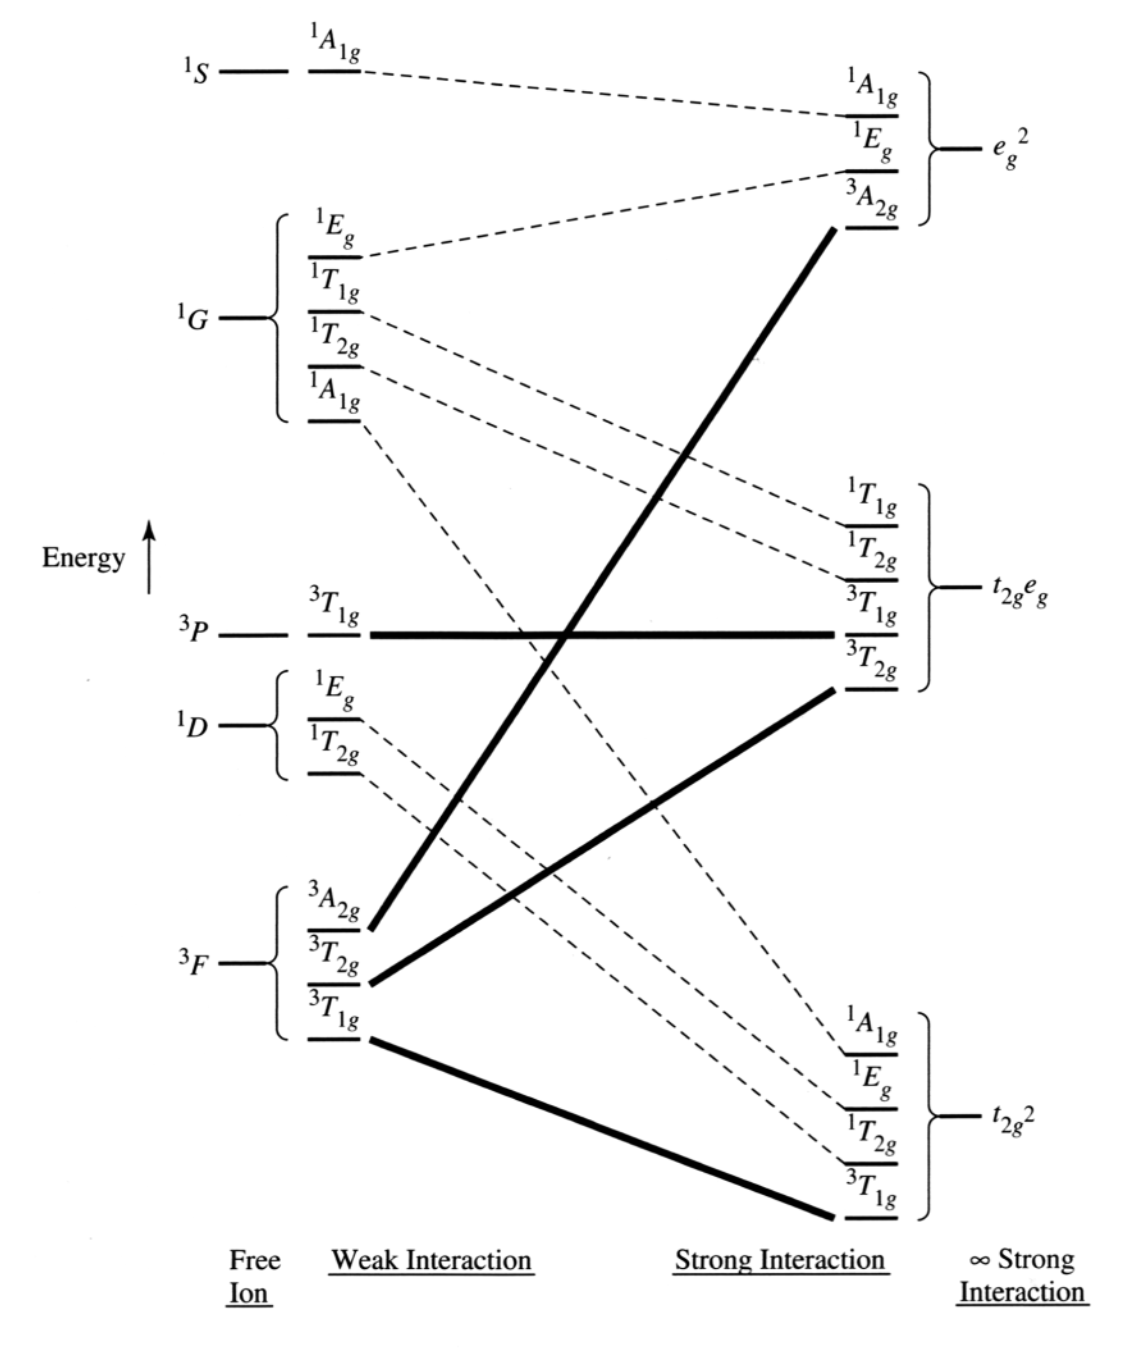
\includegraphics[width=0.45\linewidth]{../ExtFiles/correlationDiagram-d2.png}
        \caption{Correlation diagram for a $d^2$ system.}
        \label{fig:correlationDiagram-d2}
    \end{figure}
    \begin{itemize}
        \item Under a weak ligand field, the multielectron states split.
        \begin{itemize}
            \item From the $O_h$ character table, we can determine how each term transforms similarly to determining how each orbital transforms (however, we may need a character table with cubic, quartic, and beyond functions).
            \item For example, $S$ terms transform as $A_{1g}$, $P$ as $T_{1g}$, $D$ as $T_{2g}+E_g$, $F$ as $T_{1g}+T_{2g}+A_{2g}$, and $G$ as $A_{1g}+E_g+T_{1g}+T_{2g}$.
        \end{itemize}
        \item Under an infinitely strong field, we will return to our $t_{2g}$ / $e_g$ formalism with a low energy ${t_{2g}}^2$ state, a midlevel $t_{2g}e_g$ state (with one of the $d^2$ electrons in each level), and a high level ${e_g}^2$ state.
        \begin{itemize}
            \item From the $O_h$ group multiplication table, we can determine how each state splits under strong but finite ligand fields.
            \item For example, $E_g\otimes E_g=A_{1g}+E_g+A_{2g}$, so thats why the $e_g^2$ state coalesces from these three states.
        \end{itemize}
        \item The bold lines in Figure \ref{fig:correlationDiagram-d2} correspond to triplet states, and the dashed lines to singlet states.
    \end{itemize}
    \item The direct product of two irreducible representations of dimension 2 or higher is reducible to a sum of symmetric and antisymmetric irreducible representations, so named because their respective symmetry-adapted basis functions are either symmetric or antisymmetric with respect to exchange of the components. It is important to understand these properties when dealing with the electronic states produced by incompletely filled degenerate orbitals.
    \begin{itemize}
        \item The following expressions may be applied to determine the characters ($\chi$) of the symmetric and antisymmetric components of a direct product. The characters of the symmetric irreducible representation(s) ($\chi^+$) are given by
        \begin{equation*}
            \chi^+(R) = \frac{1}{2}\left( [\chi(R)]^2+\chi(R^2) \right)
        \end{equation*}
        The characters of the antisymmetric irreducible representation(s) are given by
        \begin{equation*}
            \chi^-(R) = \frac{1}{2}\left( [\chi(R)]^2-\chi(R^2) \right)
        \end{equation*}
        In these expressions, $\chi(R)$ is the character under symmetry operation $R$ and $\chi(R^2)$ is the character associated with the operation $R^2$.
        \begin{itemize}
            \item We do not need to know these formulas since deriving them is outside the scope of this course.
        \end{itemize}
        \item For example, in the $C_{4v}$ point group, the direct product $E\otimes E=A_1+A_2+B_1+B_2$.
        \item These results are typically written showing the antisymmetric component in square brackets, i.e., $E\otimes E=A_1+[A_2]+B_1+B_2$.
        \item The electron wave function, which is a product of the orbital and spin wave function components, must be antisymmetric (see Pauli exclusion principle). Therefore, if the orbital component is symmetric, the spin one should be antisymmetric, i.e., singlet state. And vice versa.
    \end{itemize}
    \item Back to our $d^2$ example:
    \begin{itemize}
        \item Symmetric components have electrons with opposite spins; antisymmetric components have electrons with like spin.
        \begin{itemize}
            \item This demonstrates how $T_2\otimes T_2=A_1+E+[T_1]+T_2$ rationalizes the existence of three singlet states and one triplet state under ${t_{2g}}^2$.
        \end{itemize}
    \end{itemize}
    \item Correlation diagrams are immensely useful, and we can tediously construct them or find them in the textbook. However, we can nicely simplify them into Tanabe-Sugano diagrams:
\end{itemize}
\begin{tchart}{1.4}{Correlation Diagram}{Tanabe-Sugano Diagram}
    Number of states. & Number of states.\\
    General sense of field effects. & Field effects.\\
    Only qualitative. & Quantitative.
\end{tchart}
\begin{itemize}
    \item Tanabe-Sugano diagrams are designed to intuitively interpret optical spectra and electron transitions in transition metal complexes.
    \item In a Tanabe-Sugano diagram, we make the lowest line in the corresponding correlation diagram the $x$-axis/ground state and calculate energies of every state above with respect to the gap between the ground state and the upper state.
    \item Tanabe-Sugano diagrams show:
    \begin{figure}[h!]
        \centering
        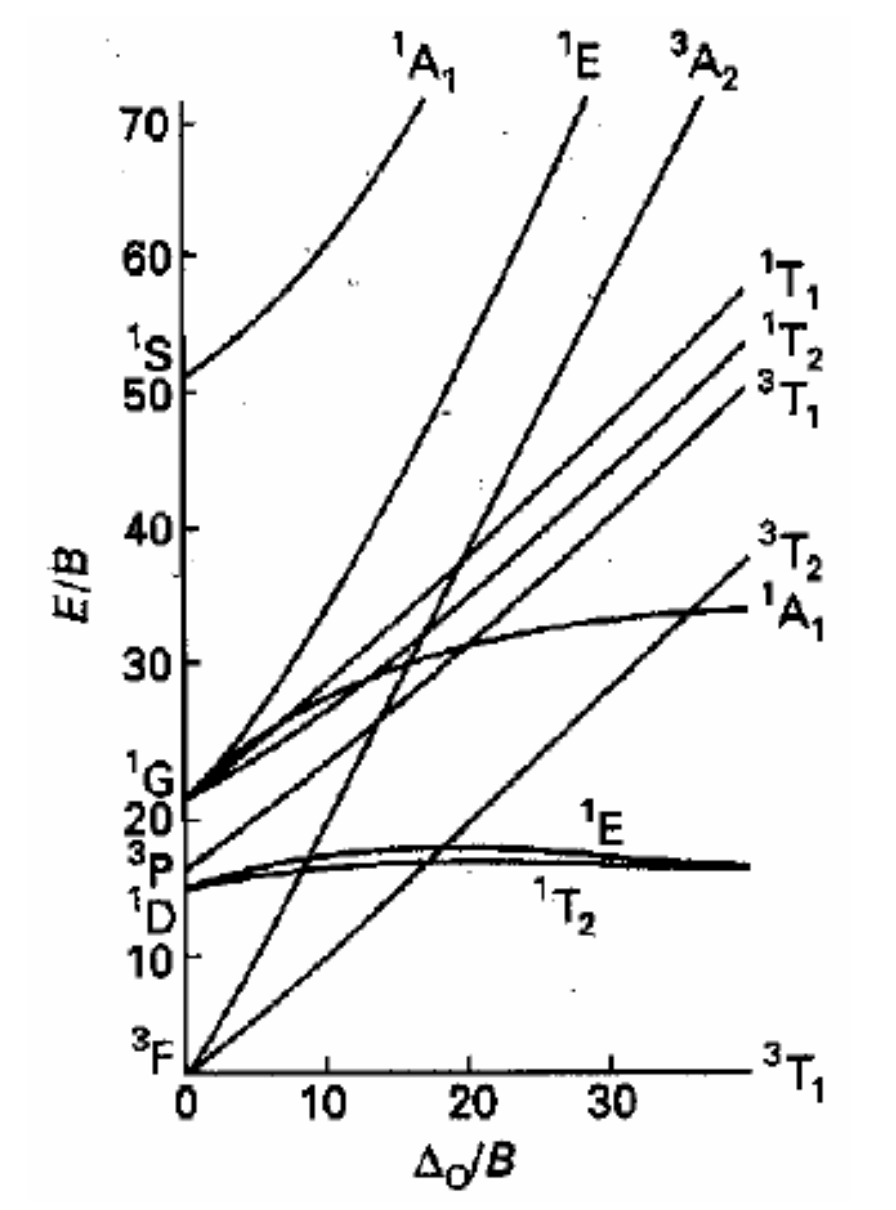
\includegraphics[width=0.35\linewidth]{../ExtFiles/tanabeSugano-d2.png}
        \caption{Tanabe-Sugano diagram for a $d^2$ system.}
        \label{fig:tanabeSugano-d2}
    \end{figure}
    \begin{itemize}
        \item Relative energies of the states vs. ligand field strength.
        \item Electronic states with the same symmetry never cross (\textbf{non-crossing rule}).
        \item Curvature (${}^1E$ and ${}^1E$).
        \item Ground state on the $x$-axis; all other states are excited.
        \item Transitions between states.
        \item A Tanabe-Sugano diagram is a graph which plots the energy of different spectroscopic terms (on the $y$-axis) against the strength of the ligand field (on the $x$-axis). The units used for each are given in terms of the \textbf{Racah parameter} $B$.
        \item The choice of unit means that the diagram takes account of electron-electron repulsion effects.
        \item The lowest energy state is usually placed along the $x$-axis.
        \item The electrostatic repulsion between electrons varies from atom to atom, depending upon the number and spin of the electrons and the orbitals they occupy. The total repulsion can be expressed in terms of three parameters $A$, $B$, and $C$, which are known as the Racah parameters. They are generally obtained empirically from gas-phase spectroscopic studies of atoms.
    \end{itemize}
    \item Each particular coordination compound will be a vertical slice through its electron configuration's Tanabe-Sugano diagram.
\end{itemize}



\section{Module 43: Using Tanabe-Sugano Diagrams}
\begin{itemize}
    \item \marginnote{3/5:}Suggested reading: Chapter 11.3.
    \item Extra Tanabe-Sugano facts:
    \begin{itemize}
        \item States of the complex have the same spin multiplicity as the free ion states from which they originate.
        \item States that are the only ones of their type have energies that depend linearly on the crystal field strength, whereas when there are two or more states of identical designation, their lines will in general show curvature. This is because such states interact with one another.
    \end{itemize}
    \item Selection rules determine the probability (intensity) of the transition.
    \item \textbf{Symmetry selection rule}: The initial and final wavefunctions must change in parity. Parity is related to the orbital angular momentum summation over all electrons $\sum {m_l}_i$, which can be even or odd; only even ($g$) $\leftrightarrow$ odd ($u$) transitions are allowed. Transitions between the orbitals of the same subshell are forbidden. \emph{Also known as} \textbf{Laporte selection rule}, \textbf{Parity selection rule}.
    \begin{itemize}
        \item For example, $g\to g$ and $u\to u$ are forbidden, but $g\to u$ and $u\to g$ are allowed.
        \item The weaker of the two selection rules.
        \item This is related back to Fermi's golden rule and $\vec{M}_{21}$.
        \item For $O_h$ complexes, $\Gamma_{\mu_{xyz}}=T_{1u}$.
        \item Direct product rules:
        \begin{align*}
            g\otimes u &= u&
            g\otimes g &= g&
            u\otimes u &= g
        \end{align*}
        \item For example, if we try a $g\to g$ transition in an $O_h$ complex, we would have $\vec{M}_{21}=g\otimes u\otimes g=u$ is unsymmetric to inversion, meaning that there is no totally symmetric representation in $\vec{M}_{21}$.
    \end{itemize}
    \item Octahedral vs. tetrahedral absorption spectra:
    \begin{itemize}
        \item A tetrahedron has no center of symmetry, and so orbitals in this point group cannot be gerade. Hence, the $d$-levels in a tetrahedral complex are $e$ and $t_2$, with no "$g$" for gerade. This largely overcomes the Laporte selection rule, making tetrahedral complexes very intense in color.
        \item This is why a solution of \ce{[Co(H2O)6]^2+} is pale pink, but \ce{[CoCl4]^2-} is a very intense blue.
    \end{itemize}
    \item \textbf{Spin selection rule}: There must be no change in the spin multiplicity ($\Delta S=0$) during the transition. i.e., the spin of the electron must not change during the transition.
    \begin{itemize}
        \item For example, ${}^1T_1\to{}^1T_2$ is allowed, but ${}^1T_1\to{}^3T_1$ and ${}^3T_1\to{}^1A_2$ are forbidden.
        \item The stronger of the two selection rules.
    \end{itemize}
    \item All $d$-$d$ transitions are symmetry (Laporte) forbidden.
    \begin{itemize}
        \item Thus, it makes more sense to disregard the complete Tanabe-Sugano diagram and focus on the spin-only one.
    \end{itemize}
    \item Example: $d^8$ Tanabe-Sugano Diagram and \ce{[Ni(H2O)6]^2+} absorption spectrum.
    \begin{figure}[h!]
        \centering
        \begin{subfigure}[b]{0.45\linewidth}
            \centering
            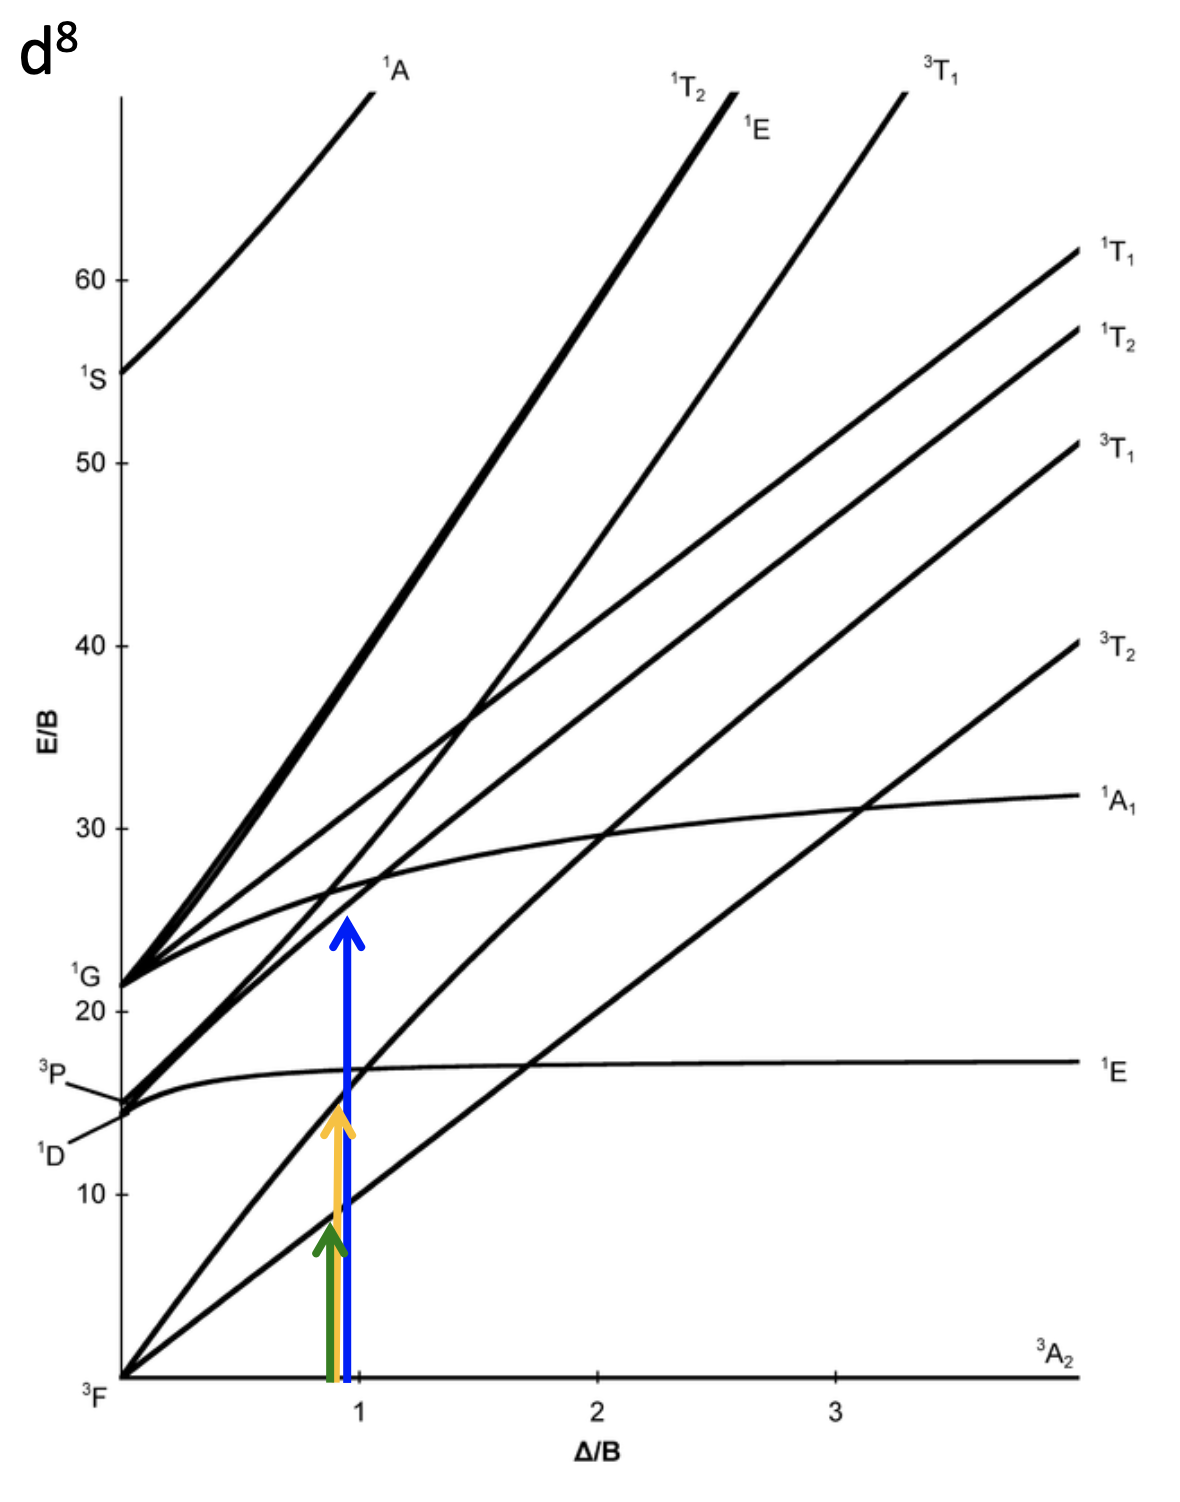
\includegraphics[width=0.8\linewidth]{../ExtFiles/NiH2O6a.png}
            \caption{The $d^8$ Tanabe-Sugano diagram.}
            \label{fig:NiH2O6a}
        \end{subfigure}
        \begin{subfigure}[b]{0.45\linewidth}
            \centering
            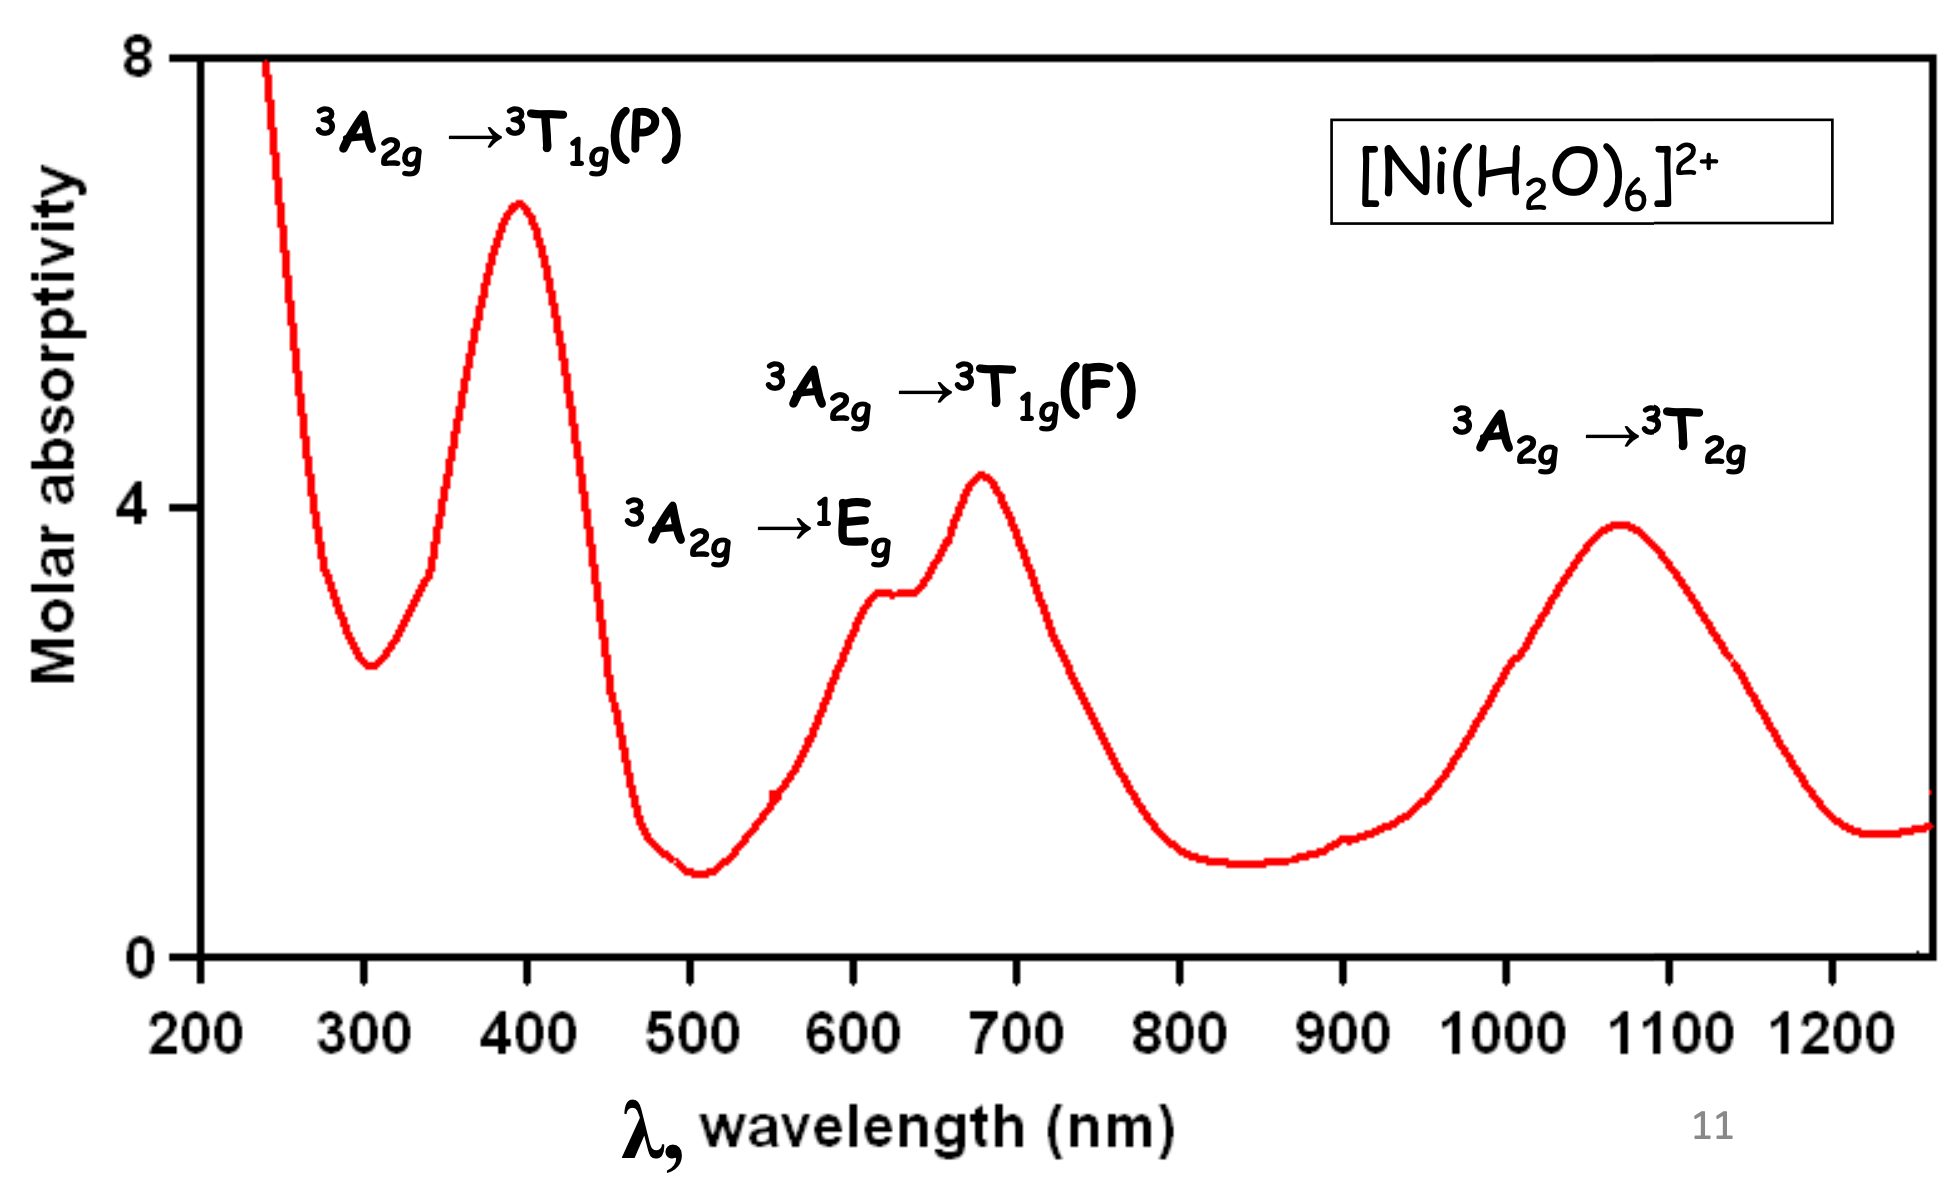
\includegraphics[width=0.95\linewidth]{../ExtFiles/NiH2O6b.png}
            \caption{The absorption spectrum.}
            \label{fig:NiH2O6b}
        \end{subfigure}
        \caption{\ce{[Ni(H2O)6]^2+}: Relating a Tanabe-Sugano diagram and an absorption spectrum.}
        \label{fig:NiH2O6}
    \end{figure}
    \begin{itemize}
        \item The two higher energy peaks involve differences in the magnetic quantum numbers of the $d$ orbitals, and are labeled as ${}^3A_{2g}\to{}^3T_{1g}(F)$ and ${}^3A_{2g}\to{}^3T_{1g}(P)$ to reflect this.
        \item Note that there is a shoulder near the second band corresponding to a nominally forbidden transition.
    \end{itemize}
    \item $d^1$ and $d^9$ complexes have only one electron transition and, thus, one peak in the absorption spectrum.
    \begin{itemize}
        \item However, the peak is not symmetric; this is a result of the Jahn-Teller distortion of the excited state.
    \end{itemize}
    \item Analyzes a ruby's Tanabe-Sugano diagram and spectrum.
    \item The $d^6$ Tanabe-Sugano diagram:
    \begin{itemize}
        \item The curves are not everywhere differentiable, the ground state changes, there is a vertical line, etc.
        \item This is because at the line, the complex switches from high-spin to low spin (recall that increasing ligand field strength increases $\Delta$; increasing $\Delta$ enough will make it larger than the spin-pairing energy).
    \end{itemize}
    \item The colors of the electron transitions tell us where the compound falls along the $x$-axis in the Tanabe-Sugano diagram.
    \item In the $d^5$ high-spin configuration, any transition involves spin pairing and does not change parity. Thus, there is a very low probability of transitions occurring.
    \item In $d^n$ and $d^{10-n}$ complexes, the splitting order in the Tanabe-Sugano diagrams (as we increase ligand field strength) is inverted.
    \begin{itemize}
        \item For example, in $d^2$, ${}^3F$ splits into (from lowest to highest energy) ${}^3T_1(F)$, ${}^3T_2$, and ${}^3A_2$. In $d^8$, ${}^3F$ splits into (from lowest to highest energy) ${}^3A_2$, ${}^3T_2$, and ${}^3T_1(F)$.
    \end{itemize}
    \item Other factors that can influence whether or not electrons are promoted:
    \begin{itemize}
        \item In $d^2$ complexes, there are three allowed transitions. However, one of them would involve promotion of two electrons from $t_{2g}$ to $e_g$ simultaneously upon the absorption of one photon, and this is highly improbable.
    \end{itemize}
    \item By comparing the energies of multiple transitions, we can look for a place in the Tanabe-Sugano diagram that would produce such results.
    \begin{itemize}
        \item For example, if one known transition has 1.5 times the energy of another, we can look for a place where the distance between it and the ground state is 1.5 times that of the other.
    \end{itemize}
    \item We can also use experimental values to calculate $B$, the Racah parameter.
    \begin{itemize}
        \item With the Racah parameter, we can pretty much calculate anything we want.
    \end{itemize}
\end{itemize}



\section{Module 44: How Can We See "Forbidden" Transitions?}
\begin{itemize}
    \item \textbf{Oscillator strength}: A quantity proportional to the integral of $\varepsilon$ as measured in the absorption spectrum. \emph{Also known as} $\bm{f}$.
    \begin{itemize}
        \item $f$ relates $\varepsilon$ to the matrix element $\vec{M}_{21}$:
        \begin{equation*}
            \frac{4m_e\pi v}{3e^2\hbar}\cdot|\vec{M}_{21}|^2 = f \propto \num{4.3e-9}\int\varepsilon\dd{\bar{\nu}}
        \end{equation*}
        \item Thus, the probability of light absorption is related to $f$.
        \item Strong absorption occurs when $f$ is around 1.
        \item The rate constant $k^0_e$ for emission is related to $\varepsilon$ by
        \begin{equation*}
            k^0_e \propto \num{4.3e-9}\bar{\nu}^{-2}_0\int\varepsilon\dd{\bar{\nu}} = \bar{\nu}^{-2}_0f
        \end{equation*}
        \begin{itemize}
            \item Good emitters are also good absorbers.
        \end{itemize}
    \end{itemize}
    \item Allowed transitions:
    \begin{itemize}
        \item Allowedness is measured by $f$ which can be dissected into
        \begin{equation*}
            f = (f_e\times f_v\times f_s)f_\text{max}
        \end{equation*}
        where $f_e$ is related to electronic factors, $f_v$ is related to Franck-Condon factors, and $f_s$ is related to spin-orbit factors.
        \item A perfectly allowed transition has $f=1$.
        \item $f_s$ factors:
        \begin{itemize}
            \item A spin-allowed transition has $f_s=1$.
            \item For a spin-forbidden transition, $f_s$ depends on spin-orbit coupling.
        \end{itemize}
        \item $f_e$ factors: \textbf{overlap forbiddenness} and \textbf{orbital forbiddenness}.
    \end{itemize}
    \item \textbf{Overlap forbiddenness}: Poor spatial overlap of orbitals involved in electronic transitions.
    \item \textbf{Orbital forbiddenness}: Wavefunctions which overlap in space but cancel because of symmetry.
    \item Mechanisms that make forbidden electronic transitions allowed: \textbf{vibronic coupling}, \textbf{spin-orbit coupling}, and \textbf{mixing of states}.
    \item \textbf{Vibronic coupling}: Electronic states coupled to vibrational states help overcome the Laporte selection rule.
    \begin{figure}[h!]
        \centering
        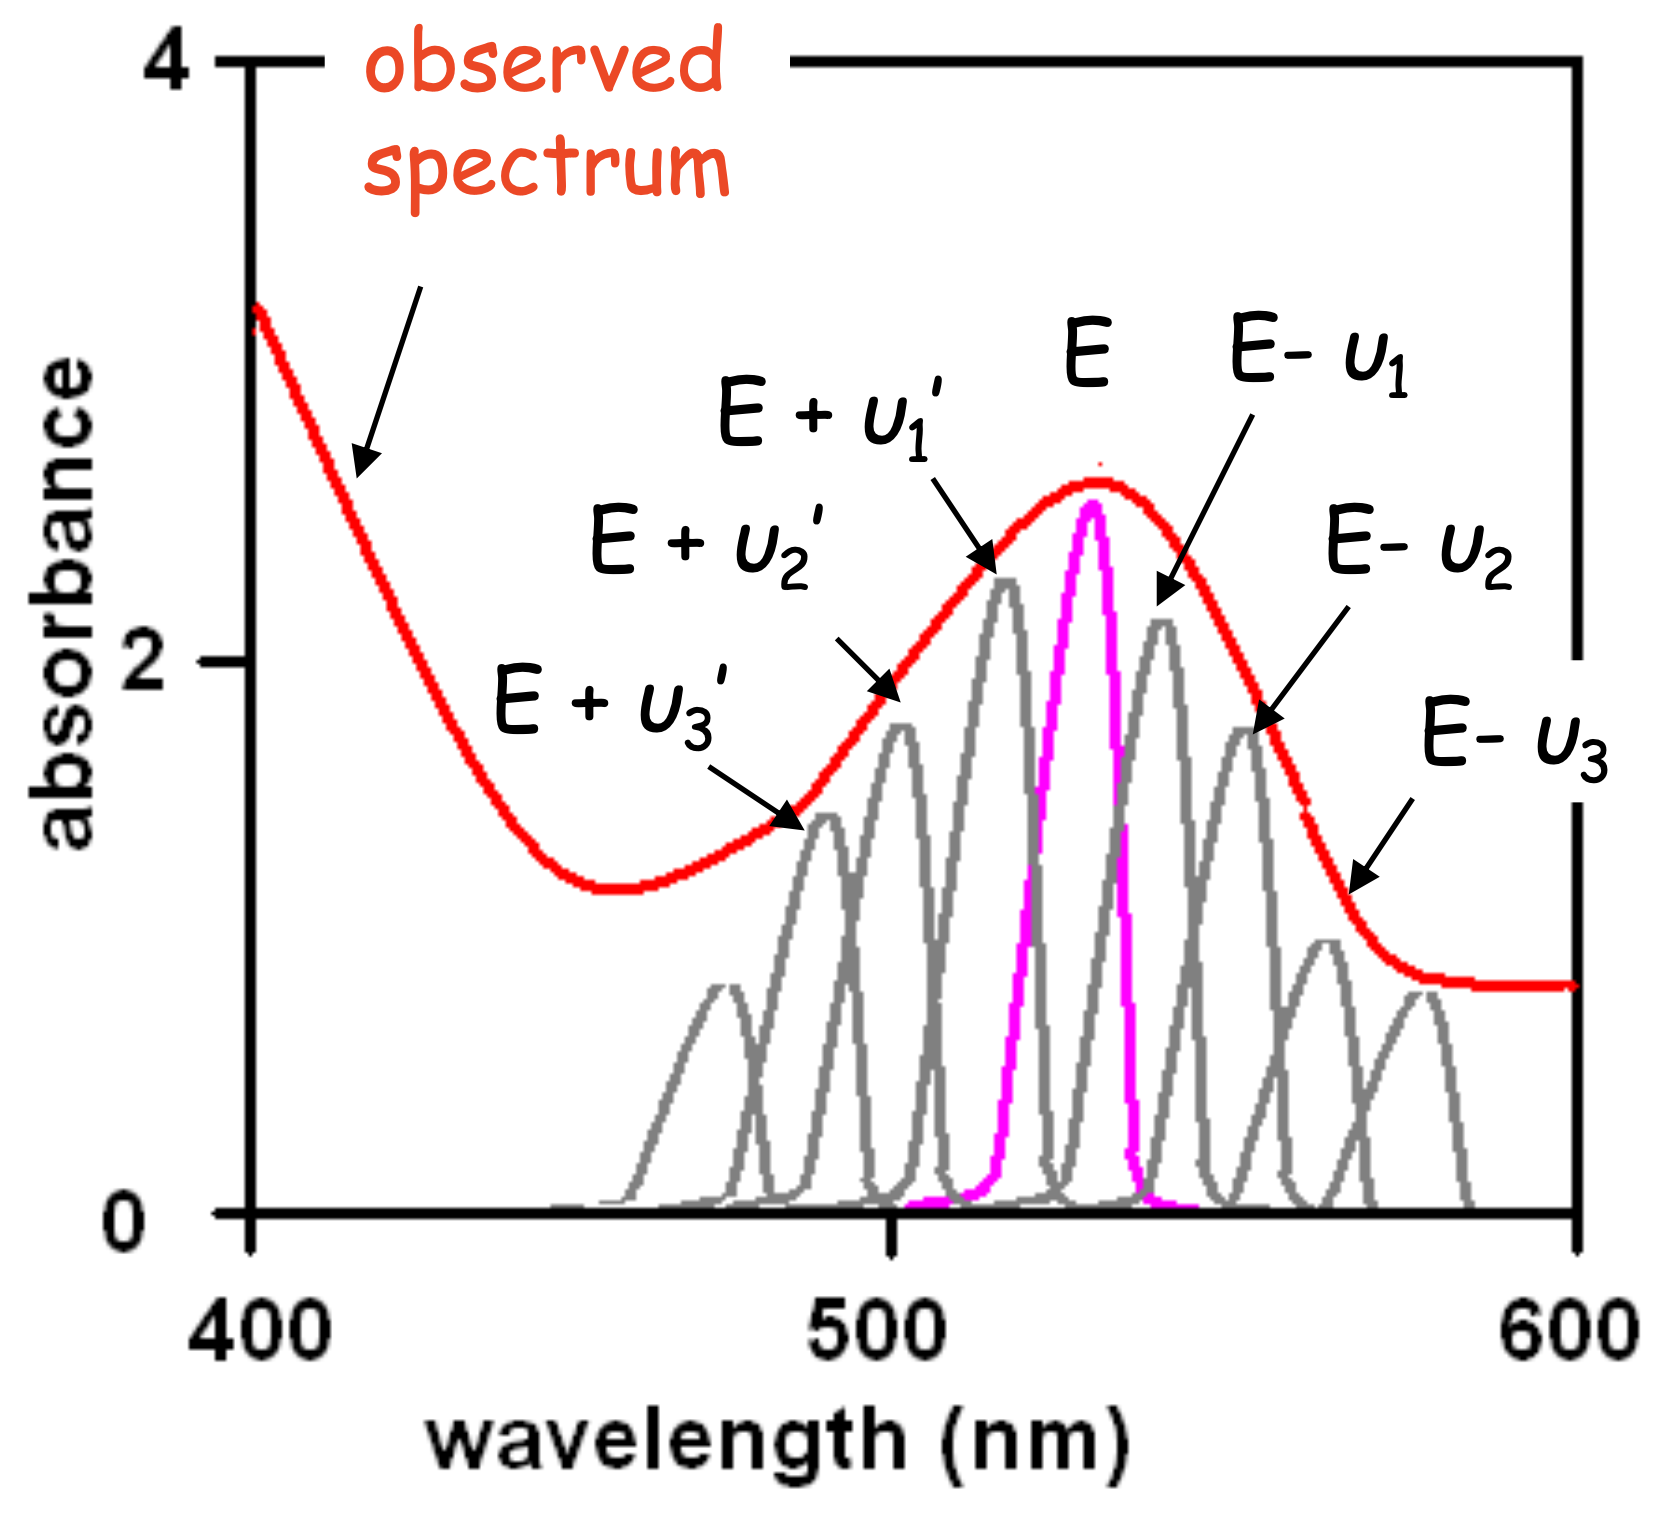
\includegraphics[width=0.3\linewidth]{../ExtFiles/vibronicCoupling.png}
        \caption{Vibronic coupling.}
        \label{fig:vibronicCoupling}
    \end{figure}
    \begin{itemize}
        \item For an octahedral complex, there are 15 vibrational normal modes with irreducible representations: $\Gamma_\text{vibs}=a_{1g}+e_g+2t_{1u}+t_{2g}+t_{2u}$.
        \item Vibrational transitions couple with electronic transition: $\vec{M}_{21}=\int\psi_v^*\psi_e^*\vec{\mu}\psi_e\psi_v\dd{\tau}$. Indeed, the wavefunction of the complex can be represented by this product (this is called the \textbf{Franck-Condon principle}), which will give fully symmetric irreducible representations.
        \item Essentially, $T_{1u}$ and $T_{2u}$ vibrations can couple with the electronic transition to form the allowed vibronic transition.
        \item The band one sees in the UV-visible spectrum is the sum of bands due to transitions too coupled electronic ($E$) and vibrational energy levels ($u_1$, $u_2$, $u_3$, etc.).
    \end{itemize}
    \item \textbf{Spin-orbit coupling}: Spin and orbital angular momenta can interact to make spin forbidden transitions allowed.
    \begin{itemize}
        \item Allows us to relax spin selection rules and promote an electron from an electron pair \emph{without changing its spin}.
        \item This is possible in heavy atoms because of their relativistic properties.
    \end{itemize}
    \item \textbf{Mixing of states}: $\pi$-acceptor and $\pi$-donor ligands can mix with the $d$-orbitals; transitions are no longer purely $d$-$d$.
    \begin{itemize}
        \item The Tanabe-Sugano diagram assumes pure $d$-$d$ transitions.
        \item However, spin-forbidden transitions can borrow intensity from nearby spin-allowed transitions by mixing of states.
    \end{itemize}
    \item $\varepsilon_\text{max}(\si{M^{-1}.cm^{-1}})$ ranges for different transitions:
    \begin{itemize}
        \item Spin and symmetry forbidden $d$-$d$ bands: 0.02-1.
        \item Spin allowed and symmetry forbidden $d$-$d$ bands: 1-10.
        \item Spin and symmetry allowed CT bands: $\num{e3}$-$\num{5e4}$.
    \end{itemize}
\end{itemize}



\section{Module 45: Charge Transfer Transitions}
\begin{itemize}
    \item \textbf{Charge-transfer band}: A Laporte- and spin-allowed, very intense absorption peak. \emph{Also known as} \textbf{CT band}.
    \item We can have transitions from metal $d$ orbitals to $p$ orbitals ($t_{2g}\to t_{1u}$).
    \begin{figure}[h!]
        \centering
        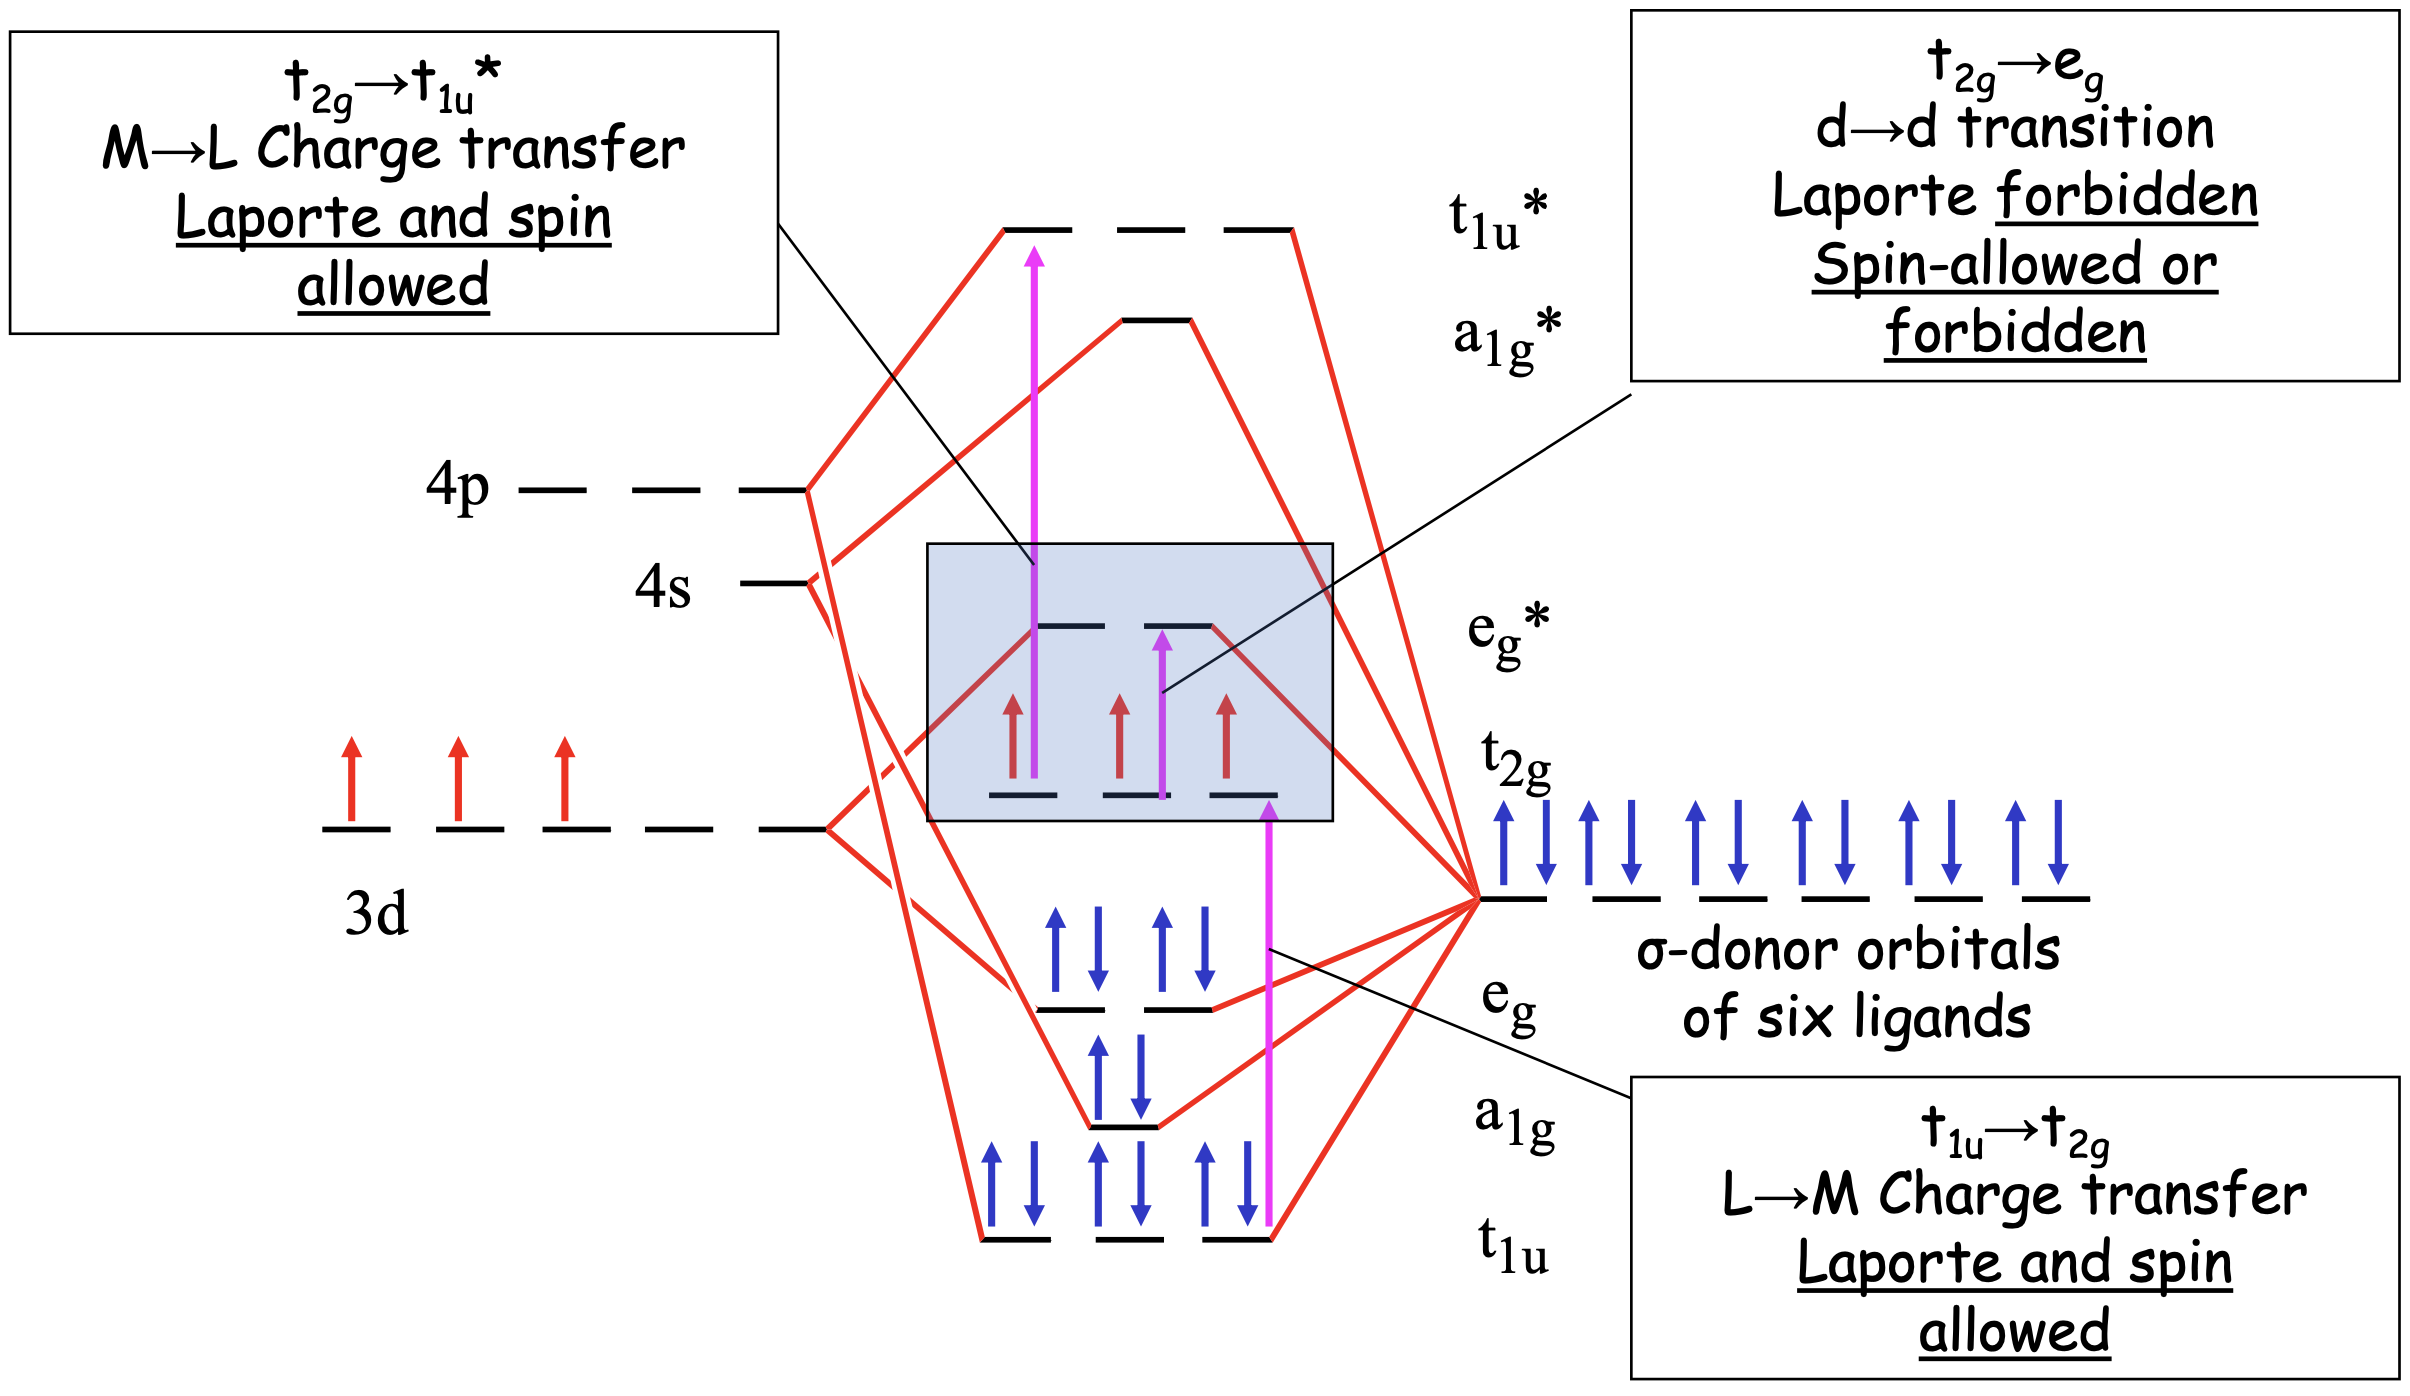
\includegraphics[width=0.8\linewidth]{../ExtFiles/chargeTransferTransitions.png}
        \caption{Electronic transitions in an octahedral complex.}
        \label{fig:chargeTransferTransitions}
    \end{figure}
    \item There exist \ce{M -> L} and \ce{L -> M} charge transfer transitions.
\end{itemize}




\end{document}